% =============================================================================
%  BÁO CÁO BÀI TẬP LỚN — CÁ NHÂN
%  Hệ thống IoT giám sát đất và không khí, điều khiển tưới tiêu theo thời gian thực
%  ESP32 + DHT22 + Potentiometer + MQTT + Node-RED Dashboard
%  Sinh viên: Phan Bá Đủ — MSSV: 22T1020073 — Lớp: TIN4024.009
% =============================================================================
\documentclass[13pt, a4paper]{article}

% =============================================================================
% 1. TIẾNG VIỆT (XeLaTeX)
% =============================================================================
\usepackage{fontspec}
\usepackage{polyglossia}
\setmainlanguage{vietnamese}
\setotherlanguage{english}

\setmainfont{Times New Roman}
\setsansfont{Arial}
\setmonofont{Courier New}

% =============================================================================
% 2. MARGIN & PAGE
% =============================================================================
\usepackage{geometry}
\geometry{
  a4paper,
  top    = 2.0cm,
  bottom = 2.0cm,
  left   = 3.0cm,
  right  = 2.0cm
}

\usepackage{setspace}
\onehalfspacing

% =============================================================================
% 3. TIỆN ÍCH
% =============================================================================
\usepackage{hyperref}
\usepackage{graphicx}
\graphicspath{{./images/}}
\usepackage{float}
\usepackage{booktabs}
\usepackage{array}
\usepackage{tabularx}
\newcolumntype{C}[1]{>{\centering\arraybackslash}p{#1}}
\newcolumntype{L}[1]{>{\raggedright\arraybackslash}p{#1}}
\usepackage{longtable}
\usepackage{seqsplit}
\usepackage{enumitem}
\usepackage{titlesec}
\usepackage{tocloft}
\usepackage{fancyhdr}
\usepackage{xcolor}
\usepackage{listings}
\usepackage{ifthen}
\usepackage{amssymb}
\usepackage[nottoc,notlof,notlot]{tocbibind}
\usepackage{placeins}
\usepackage{tikz}
\usetikzlibrary{positioning,arrows.meta,calc}

% Cấu hình listings (mã nguồn C++)
\lstset{
  basicstyle   = \ttfamily\small,
  keywordstyle = \color{blue}\bfseries,
  commentstyle = \color{gray}\itshape,
  stringstyle  = \color{orange},
  breaklines   = true,
  frame        = single,
  numbers      = left,
  numberstyle  = \tiny\color{gray},
  captionpos   = b
}

\lstdefinestyle{ccode}{
    language=C++,
    backgroundcolor=\color{white},
    commentstyle=\color{gray}\itshape,
    keywordstyle=\color{blue}\bfseries,
    stringstyle=\color{orange},
    numberstyle=\tiny\color{gray},
    basicstyle=\ttfamily\small,
    breaklines=true,
    frame=single,
    numbers=left,
    numbersep=5pt,
    stepnumber=1,
    tabsize=4,
    keepspaces=true,
    showstringspaces=false,
    captionpos=b,
    xleftmargin=10pt
}

\lstdefinestyle{jcode}{
    language=Java,
    backgroundcolor=\color{white},
    commentstyle=\color{gray}\itshape,
    keywordstyle=\color{violet!55!black}\bfseries,
    stringstyle=\color{blue!35!black},
    numberstyle=\tiny\color{gray},
    basicstyle=\ttfamily\small,
    breaklines=true,
    frame=single,
    numbers=left,
    numbersep=5pt,
    stepnumber=1,
    tabsize=4,
    keepspaces=true,
    showstringspaces=false,
    captionpos=b,
    xleftmargin=10pt
}

% =============================================================================
% 4. SỐ TRANG
% =============================================================================
\pagestyle{fancy}
\fancyhf{}
\cfoot{\thepage}
renewcommand{\headrulewidth}{0pt}

\hypersetup{
  unicode    = true,
  colorlinks = true,
  linkcolor  = black,
  citecolor  = black,
  urlcolor   = blue
}

% =============================================================================
% 5. ĐỊNH NGHĨA MACRO
% =============================================================================
\newcommand{\code}[1]{\texttt{\detokenize{#1}}}
\newcommand{\file}[1]{\textbf{\texttt{\detokenize{#1}}}}
\newcommand{\codebreak}[1]{\texttt{\seqsplit{#1}}}
renewcommand{\contentsname}{MỤC LỤC}

% =============================================================================
% ========================  NỘI DUNG TÀI LIỆU  ============================
% =============================================================================
\begin{document}

% =============================================================================
% TRANG BÌA
% =============================================================================
\thispagestyle{empty}
\begin{center}
  \fontsize{18}{22}\selectfont\bfseries
  ĐẠI HỌC HUẾ\\
  TRƯỜNG ĐẠI HỌC KHOA HỌC\\[0.4cm]
  
\includegraphics[width=4.5cm]{logo.png}\\[0.45cm]
  \rule{\linewidth}{0.5pt}\\[1cm]
  {\LARGE\bfseries THIẾT KẾ VÀ TRIỂN KHAI HỆ THỐNG IoT\\ GIÁM SÁT ĐẤT VÀ KHÔNG KHÍ,\\ ĐIỀU KHIỂN TƯỚI TIÊU THEO THỜI GIAN THỰC}\\[1cm]
  {\large Học phần: Phát triển ứng dụng IoT}\\
  {\large Mã học phần: TIN4024}\\[2cm]
  {\large Sinh viên thực hiện: Phan Bá Đủ}\\
  {\large MSSV: 22T1020073}\\
  {\large Lớp: TIN4024.009}\\[2cm]
  {\large Giảng viên hướng dẫn: Lê Hữu Bình}\\[3cm]
  {\large Huế, Ngày 08 Tháng 04 Năm 2026}
\end{center}

\newpage

% =============================================================================
% LỜI CẢM ƠN
% =============================================================================
\thispagestyle{empty}
\vspace*{0.4cm}
\begin{center}
  \fontsize{17}{21}\selectfont\bfseries LỜI CẢM ƠN\par
  \vspace{0.2ex}
  \rule{0.28\textwidth}{1.8pt}
\end{center}
\vspace{0.6cm}

\parindent=1.1cm
\setlength{\parskip}{0.55ex plus 0.2ex}

Trong quá trình thực hiện bài báo cáo này, em đã nhận được sự hỗ trợ, giúp đỡ tận tình từ thầy cô, bạn bè và gia đình. Em xin chân thành gửi lời cảm ơn sâu sắc đến:

\textbf{Trước hết}, em xin bày tỏ lòng biết ơn đến Thầy Lê Hữu Bình, người đã tận tình chỉ dẫn, góp ý và đồng hành cùng em trong suốt quá trình nghiên cứu và hoàn thiện bài báo cáo. Sự hướng dẫn quý báu của thầy là nguồn động lực và định hướng quan trọng giúp em hoàn thành tốt bài báo cáo này.

\textbf{Em cũng xin gửi lời cảm ơn} đến quý thầy cô trong khoa Công Nghệ Thông Tin, những người đã truyền đạt kiến thức nền tảng và tạo điều kiện thuận lợi để em có thể áp dụng vào quá trình thực tập và hoàn thiện bài báo cáo.

Mặc dù đã cố gắng hoàn thiện bài viết trong khả năng của mình, nhưng chắc chắn không thể tránh khỏi những thiếu sót. Em rất mong nhận được sự góp ý từ quý thầy cô để bài viết được hoàn thiện hơn.

Một lần nữa, em xin chân thành cảm ơn và luôn mong nhận được sự đóng góp của Quý thầy cô. Em xin kính chúc các thầy cô trong Khoa Công nghệ Thông tin dồi dào sức khỏe, niềm tin để tiếp tục thực hiện sứ mệnh cao đẹp của mình là truyền đạt kiến thức cho thế hệ mai sau.

Em xin chân thành cảm ơn!

\parindent=0pt
\parskip=0pt
\vspace{0.5cm}
\hfill\begin{minipage}[t]{7cm}
  \fontsize{13}{17}\selectfont
  \begin{flushright}
    \textbf{Phan Bá Đủ}\\
    MSSV: 22T1020073\\
    Lớp: TIN4024.009\\
    Huế, tháng 04 năm 2026
  \end{flushright}
\end{minipage}

\newpage

% =============================================================================
% DANH MỤC TỪ VIẾT TẮT
% =============================================================================
\thispagestyle{empty}
\vspace*{0.4cm}
\begin{center}
  \fontsize{17}{21}\selectfont\bfseries DANH MỤC CÁC TỪ VIẾT TẮT
\end{center}
\vspace{0.5cm}

\noindent
\begingroup
renewcommand{\arraystretch}{1.2}%
\begin{tabularx}{\textwidth}{@{}C{2.5cm}X@{}}
  \toprule
  \textbf{Ký hiệu} & \textbf{Giải thích} \\
  \midrule
  \textbf{API}   & Application Programming Interface --- Giao diện lập trình ứng dụng \\
  \textbf{ADC}   & Analog-to-Digital Converter --- Bộ chuyển đổi tương tự sang số \\
  \textbf{DHT}   & Digital Humidity and Temperature --- Cảm biến nhiệt độ và độ ẩm số \\
  \textbf{GPIO}  & General Purpose Input/Output --- Chân vào/ra đa mục đích \\
  \textbf{IoT}   & Internet of Things --- Internet vạn vật \\
  \textbf{JSON}  & JavaScript Object Notation --- Định dạng chuỗi dữ liệu khóa-giá trị \\
  \textbf{LED}   & Light-Emitting Diode --- Điốt phát quang \\
  \textbf{MQTT}  & Message Queuing Telemetry Transport --- Giao thức truyền thông pub/sub \\
  \textbf{MQTT Broker} & Phần mềm trung gian nhận và phân phối message theo topic \\
  \textbf{NRD}   & Node-RED Dashboard --- Giao diện Dashboard của Node-RED \\
  \textbf{Pub/Sub} & Publisher/Subscriber --- Mô hình gửi/nhận message qua topic \\
  \textbf{TLS}   & Transport Layer Security --- Giao thức bảo mật tầng truyền tải \\
  \bottomrule
\end{tabularx}
\endgroup

\newpage

% =============================================================================
% MỤC LỤC
% =============================================================================
\pagenumbering{gobble}
\thispagestyle{empty}
\vspace*{0.35\baselineskip}
{\setstretch{1}\normalsize
  \tableofcontents
}
\newpage

% =============================================================================
% BẮT ĐẦU ĐÁNH SỐ TRANG
% =============================================================================
\pagenumbering{arabic}
\thispagestyle{fancy}
\fontsize{13}{19.5}\selectfont

% =============================================================================
% PHẦN 1: ĐẶT VẤN ĐỀ
% =============================================================================
\section*{Đặt vấn đề}
\addcontentsline{toc}{section}{Đặt vấn đề}
\label{sec:datvande}

Ngày nay, Internet vạn vật (Internet of Things — IoT) đang ngày càng phát triển mạnh mẽ và được ứng dụng rộng rãi trong nhiều lĩnh vực khác nhau: từ điều khiển tự động trong công nghiệp, giám sát sức khỏe cá nhân, đến nông nghiệp thông minh (Smart Farming). Theo định nghĩa, IoT là mô hình cho phép các thiết bị vật lý (cảm biến, vi điều khiển) kết nối với nhau và với internet, từ đó thu thập dữ liệu, trao đổi thông tin và thực hiện các hành động điều khiển mà không cần sự can thiệp trực tiếp của con người.

Trong bối cảnh biến đổi khí hậu ngày càng gay gắt, việc sản xuất nông nghiệp đối mặt với nhiều thách thức: nắng nóng kéo dài, hạn hán cục bộ, nguồn nước ngày càng khan hiếm. Trồng cây trong nhà kính hoặc trên sân thượng đang trở thành xu hướng tại các đô thị lớn, nơi không gian đất canh tác bị thu hẹp. Tuy nhiên, việc tưới tiêu thủ công không chỉ tốn nhiều thời gian mà còn không đảm bảo cây luôn được cung cấp nước đúng lúc, đúng liều lượng.

Xuất phát từ thực tiễn đó, báo cáo này tập trung thiết kế và triển khai một hệ thống IoT giám sát đất và không khí, điều khiển tưới tiêu theo thời gian thực, với các mục tiêu cụ thể sau:

\begin{itemize}
  \item Giám sát độ ẩm đất, nhiệt độ và độ ẩm không khí theo thời gian thực.
  \item Truyền dữ liệu cảm biến lên cloud thông qua giao thức MQTT (Message Queuing Telemetry Transport) với bảo mật TLS.
  \item Cung cấp giao diện Dashboard trực quan trên trình duyệt web để giám sát và điều khiển hệ thống từ xa.
  \item Cảnh báo bằng buzzer khi đất quá khô, đồng thời hỗ trợ chế độ tưới tự động dựa trên ngưỡng độ ẩm đất.
  \item Cho phép điều khiển bật/tắt máy bơm bằng tay qua Dashboard.
\end{itemize}

Hệ thống được xây dựng với ba thành phần chính: (1) thiết bị đầu cuối dựa trên vi điều khiển ESP32 kết nối với cảm biến DHT22 (không khí) và Potentiometer (độ ẩm đất); (2) tầng trung gian là MQTT Broker HiveMQ Cloud qua giao thức bảo mật TLS (port 8883); (3) tầng ứng dụng là Node-RED Dashboard cung cấp giao diện giám sát và điều khiển trên trình duyệt web.

% =============================================================================
% PHẦN 2: NỘI DUNG THỰC HIỆN
% =============================================================================
\section{Nội dung thực hiện}
\label{sec:noidung}

\subsection{Các nội dung đã thực hiện}

Trong phạm vi đề tài, các nội dung chính đã được triển khai bao gồm:

\begin{enumerate}[label=\arabic*., leftmargin=1.5cm]
  \item \textbf{Thu thập dữ liệu môi trường:} ESP32 đọc nhiệt độ và độ ẩm không khí từ cảm biến DHT22 (GPIO 4), đọc độ ẩm đất từ Potentiometer (GPIO 34) mỗi 5 giây.
  \item \textbf{Truyền dữ liệu qua MQTT:} ESP32 đóng gói dữ liệu thành JSON và publish lên topic \code{iot/farm/env} qua HiveMQ Cloud TLS (port 8883).
  \item \textbf{Xử lý dữ liệu bằng Node-RED:} Nhận message từ MQTT, parse JSON, tách luồng hiển thị gauge, chart, cảnh báo.
  \item \textbf{Hiển thị Dashboard:} Gauge độ ẩm đất, gauge nhiệt độ, gauge độ ẩm không khí, biểu đồ line theo thời gian thực.
  \item \textbf{Cảnh báo:} Toast thông báo khi đất khô ($<$ 30\%); cảnh báo buzzer khi đất quá khô ($<$ 20\%); toast khi nhiệt độ cao ($>$ 35$^\circ$C).
  \item \textbf{Điều khiển bơm từ Dashboard:} Nút bật/tắt bơm, công tắc tưới tự động, gửi lệnh qua MQTT topic \code{iot/farm/control}.
  \item \textbf{Xử lý lệnh điều khiển trên ESP32:} Callback MQTT nhận lệnh bật/tắt bơm, cập nhật trạng thái LED và buzzer.
  \item \textbf{Mô phỏng trên Wokwi:} Sơ đồ mạch hoàn chỉnh với ESP32, DHT22, Potentiometer, LED và Buzzer.
\end{enumerate}

% -----------------------------------------------------------------------------
\subsection{Thiết kế mạch IoT}

\subsubsection{Sơ đồ logic của hệ thống}

Hệ thống được thiết kế theo mô hình ba tầng, mỗi tầng đảm nhiệm một chức năng riêng biệt và giao tiếp với tầng trên/dưới qua giao diện xác định.

Tầng thứ nhất là \textbf{tầng thiết bị đầu cuối (Device Layer)}: ESP32 kết nối với cảm biến DHT22 qua chân GPIO 4 để đọc nhiệt độ và độ ẩm không khí; kết nối Potentiometer qua chân GPIO 34 (ADC) để đọc độ ẩm đất; điều khiển LED (mô phỏng máy bơm) qua GPIO 5 và buzzer qua GPIO 27.

Tầng thứ hai là \textbf{tầng mạng (Network Layer)}: HiveMQ Cloud nhận message từ ESP32 qua topic \code{iot/farm/env} (dữ liệu cảm biến) và phân phối cho các subscriber; đồng thời nhận lệnh điều khiển từ Node-RED qua topic \code{iot/farm/control}.

Tầng thứ ba là \textbf{tầng ứng dụng (Application Layer)}: Node-RED nhận dữ liệu, xử lý theo logic, hiển thị lên Dashboard và gửi lệnh điều khiển xuống ESP32.

\begin{figure}[H]
  \centering
  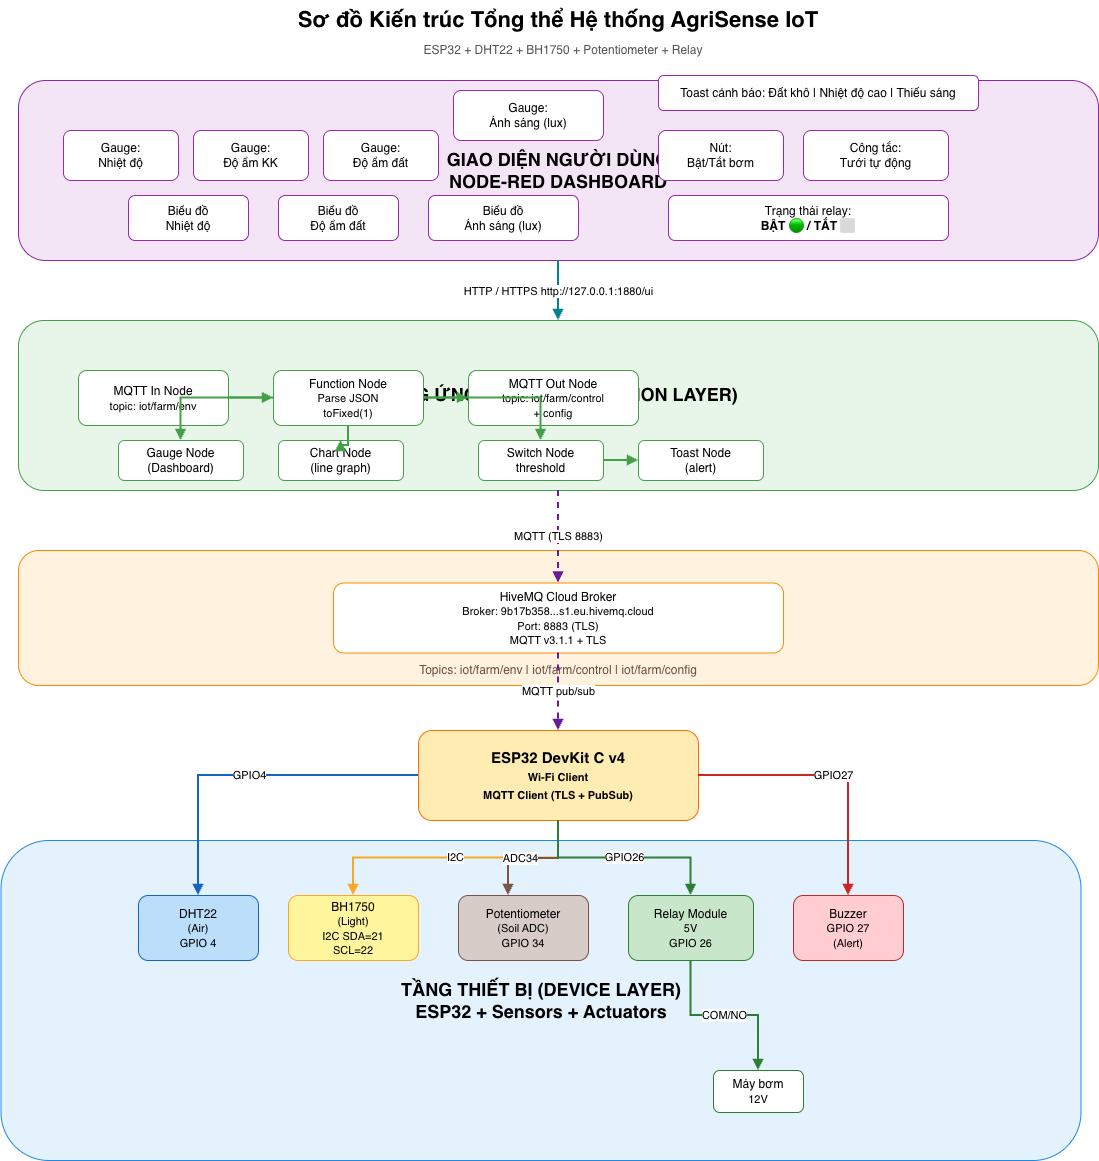
\includegraphics[width=0.88\linewidth]{so-do-kien-truc-he-thong.png}
  \caption{Sơ đồ kiến trúc tổng thể hệ thống AgriSense IoT}
  \label{fig:kien-truc}
\end{figure}

Sơ đồ kết nối phần cứng trên Wokwi:

\begin{figure}[H]
  \centering
  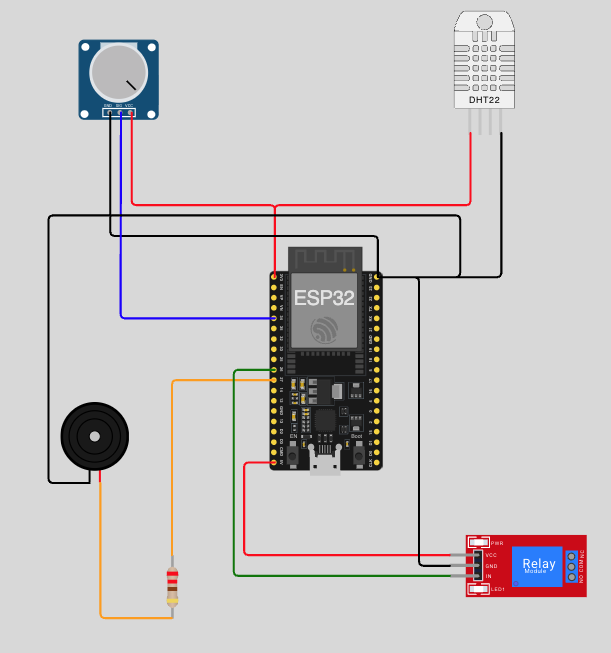
\includegraphics[width=0.88\linewidth]{mach-vat-ly-wokwi.png}
  \caption{Mạch mô phỏng Wokwi: ESP32 DevKit C v4 + DHT22 + Potentiometer + LED + Buzzer}
  \label{fig:wokwi}
\end{figure}

\subsubsection{Chức năng cơ bản của các linh kiện, thiết bị}

\textbf{1) ESP32 (DevKit C v4)}

ESP32 là vi điều khiển do Espressif Systems phát triển, nổi bật với khả năng tích hợp Wi-Fi 802.11 b/g/n và Bluetooth BR/EDD dual-mode trên cùng một chip. Về phần cứng, ESP32 sử dụng CPU dual-core Xtensa LX6 với tần số lên tới 240 MHz, có SRAM 520 KB, hỗ trợ GPIO đa chức năng, ADC 12-bit, DAC, SPI, I2C, UART. Việc lập trình ESP32 có thể thực hiện qua PlatformIO trên VS Code, với hệ sinh thái thư viện phong phú.

Trong đề tài này, ESP32 đảm nhiệm các chức năng chính: (1) kết nối Wi-Fi để truyền dữ liệu; (2) giao tiếp với cảm biến DHT22 qua chân GPIO 4 để đọc nhiệt độ và độ ẩm không khí; (3) đọc điện áp từ Potentiometer qua chân GPIO 34 (ADC1\_6) để tính độ ẩm đất; (4) điều khiển LED (mô phỏng máy bơm) qua chân GPIO 5; (5) điều khiển Buzzer cảnh báo qua chân GPIO 27.

So với ESP8266, ESP32 có ưu thế về bộ nhớ lớn hơn, xử lý nhanh hơn, hỗ trợ đa luồng (multi-threading) nhờ kiến trúc dual-core, và có nhiều chân ADC hơn phù hợp cho việc đọc cảm biến analog.

\textbf{2) Cảm biến DHT22 (AM2302)}

DHT22 là cảm biến đo nhiệt độ và độ ẩm không khí số, được sản xuất bởi Aosong Electronics. So với phiên bản DHT11, DHT22 có độ chính xác cao hơn đáng kể, phù hợp hơn cho các ứng dụng đòi hỏi số liệu tin cậy.

Thông số kỹ thuật của DHT22: dải đo nhiệt độ từ $-40^\circ$C đến $+80^\circ$C với sai số $\pm0.5^\circ$C; dải đo độ ẩm từ 0\% đến 100\% RH với sai số $\pm2\%$ RH; điện áp hoạt động từ 3.3V đến 5.5V; giao tiếp qua giao thức 1-wire (Single-Wire). DHT22 trả dữ liệu dạng số 40-bit: 16 bit đầu cho độ ẩm (hundreds), 16 bit tiếp cho nhiệt độ, và 8 bit cuối là checksum để kiểm tra lỗi truyền.

Cảm biến DHT22 được lựa chọn trong đề tài này thay vì DHT11 vì độ chính xác cao hơn, giá thành hợp lý, và vẫn đủ đơn giản để tích hợp trong một hệ thống IoT cơ bản.

\textbf{3) Potentiometer (Biến trở)}

Potentiometer được sử dụng trong mô phỏng Wokwi để mô phỏng cảm biến độ ẩm đất. Potentiometer kết nối với chân ADC (GPIO 34) của ESP32. Khi giá trị điện trở thay đổi (tương ứng với độ ẩm đất thay đổi), điện áp đọc được qua ADC sẽ thay đổi theo. ESP32 sử dụng bộ chuyển đổi ADC 12-bit (0--4095), giá trị được map tuyến tính về thang 0--100\% đại diện cho độ ẩm đất.

Trong thực tế, cảm biến độ ẩm đất capacitive (như vỉ FY-550 hoặc vỉ với IC v3) hoạt động tương tự: đo điện dung thay đổi theo độ ẩm đất và xuất tín hiệu analog tương ứng. Potentiometer trong mô phỏng Wokwi đóng vai trò tương đương, cho phép kiểm thử hệ thống mà không cần phần cứng thật.

\textbf{4) LED (mô phỏng máy bơm)}

LED xanh được kết nối với GPIO 5 của ESP32 thông qua điện trở hạn dòng 220$\Omega$. Trong hệ thống thực tế, LED này được thay bằng relay 5V điều khiển máy bơm nước 12V. Khi ESP32 nhận lệnh bật bơm qua MQTT, chân GPIO 5 xuất mức HIGH, LED sáng (hoặc relay đóng, máy bơm chạy).

\textbf{5) Buzzer (báo động)}

Buzzer được kết nối với GPIO 27 của ESP32 thông qua điện trở hạn dòng 220$\Omega$. Buzzer phát ra âm báo khi độ ẩm đất giảm xuống dưới ngưỡng nguy hiểm ($<$ 20\%): bíp 5 lần, mỗi lần bật 300ms và tắt 200ms. Khi đất khô nhưng chưa nguy hiểm ($<$ 30\% và $\ge$ 20\%), buzzer bíp 2 lần ngắn hơn (150ms bật, 150ms tắt) như tín hiệu nhắc nhở.

Bảng kết nối chân GPIO trên ESP32 DevKit C v4:

\begin{table}[H]
  \centering
  \caption{Bảng kết nối chân GPIO trên ESP32}
  \label{tbl:gpio}
  \begin{tabular}{|L{3.5cm}|C{3.5cm}|C{4.5cm}|}
    \hline
    \textbf{Chân ESP32} & \textbf{Nối đến} & \textbf{Chức năng} \\
    \hline
    3V3 & DHT22 VCC, Potentiometer VCC & Nguồn 3.3V cho cảm biến \\
    \hline
    GND & DHT22 GND, LED Cathode, Buzzer -, Potentiometer GND & Chân nối đất chung \\
    \hline
    GPIO 4 & DHT22 DATA & Bus dữ liệu 1-wire \\
    \hline
    GPIO 5 & LED Anode (qua R220) & Điều khiển bật/tắt LED (mô phỏng bơm) \\
    \hline
    GPIO 27 & Buzzer + (qua R220) & Điều khiển buzzer báo động \\
    \hline
    GPIO 34 & Potentiometer SIG & Đọc điện áp ADC — tính độ ẩm đất \\
    \hline
  \end{tabular}
\end{table}

\subsubsection{Nguyên lý hoạt động}

Hệ thống hoạt động theo ba luồng chính sau đây:

\textbf{Luồng 1 — Giám sát môi trường:}

\begin{enumerate}[label=\arabic*., leftmargin=1.5cm]
  \item DHT22 đo nhiệt độ và độ ẩm không khí tại chân GPIO 4.
  \item Potentiometer cung cấp điện áp analog tại chân GPIO 34 (ADC).
  \item \code{loop()} kiểm tra timer \code{lastPublish}; đủ 5000ms $\rightarrow$ gọi \code{readSensors()}.
  \item Hàm \code{readSoilMoisture()} đọc ADC (0--4095), map về thang 0--100\%.
  \item Hàm \code{publishSensorData()} đóng gói JSON: \code{\{"device","temperature","humidity","soilMoisture","pumpStatus","timestamp"\}}.
  \item \code{mqttClient.publish("iot/farm/env", buffer)} $\rightarrow$ HiveMQ Cloud.
  \item Node-RED nhận JSON $\rightarrow$ \code{HandleData} parse $\rightarrow$ gauge, chart, cảnh báo.
  \item Dashboard cập nhật giá trị đo được theo thời gian thực.
\end{enumerate}

\textbf{Luồng 2 — Cảnh báo độ ẩm đất:}

\begin{enumerate}[label=\arabic*., leftmargin=1.5cm]
  \item ESP32 so sánh \code{soilMoisture} với ngưỡng \code{SOIL_CRITICAL_THRESHOLD = 20\%}.
  \item Nếu $<$ 20\%: gọi \code{beepAlert(5, 300, 200)} — bíp 5 lần, mỗi lần 300ms bật, 200ms tắt.
  \item Nếu 20\% $\le$ soil $<$ 30\%: gọi \code{beepAlert(2, 150, 150)} — bíp 2 lần ngắn.
  \item Đồng thời, Node-RED switch node kiểm tra ngưỡng để hiển thị toast cảnh báo và cảnh báo đỏ trên Dashboard.
\end{enumerate}

\textbf{Luồng 3 — Điều khiển bơm từ Dashboard:}

\begin{enumerate}[label=\arabic*., leftmargin=1.5cm]
  \item Người dùng nhấn nút \textbf{Bật bơm} hoặc \textbf{Tắt bơm} trên Node-RED Dashboard.
  \item Node-RED gửi JSON \code{\{"pump":true,"duration":5\}} hoặc \code{\{"pump":false,"duration":0\}} lên topic \code{iot/farm/control}.
  \item ESP32 \code{mqttCallback()} nhận message, kiểm tra topic.
  \item \code{handleControlMessage()} parse JSON, kiểm tra key \code{pump}.
  \item \code{setPump(true/false)} xuất mức HIGH/LOW ra GPIO 5 $\rightarrow$ LED bật/tắt.
  \item Serial log ghi \code{[PUMP] ON/OFF}.
\end{enumerate}

Lưu đồ thuật toán trên ESP32:

\begin{figure}[H]
  \centering
  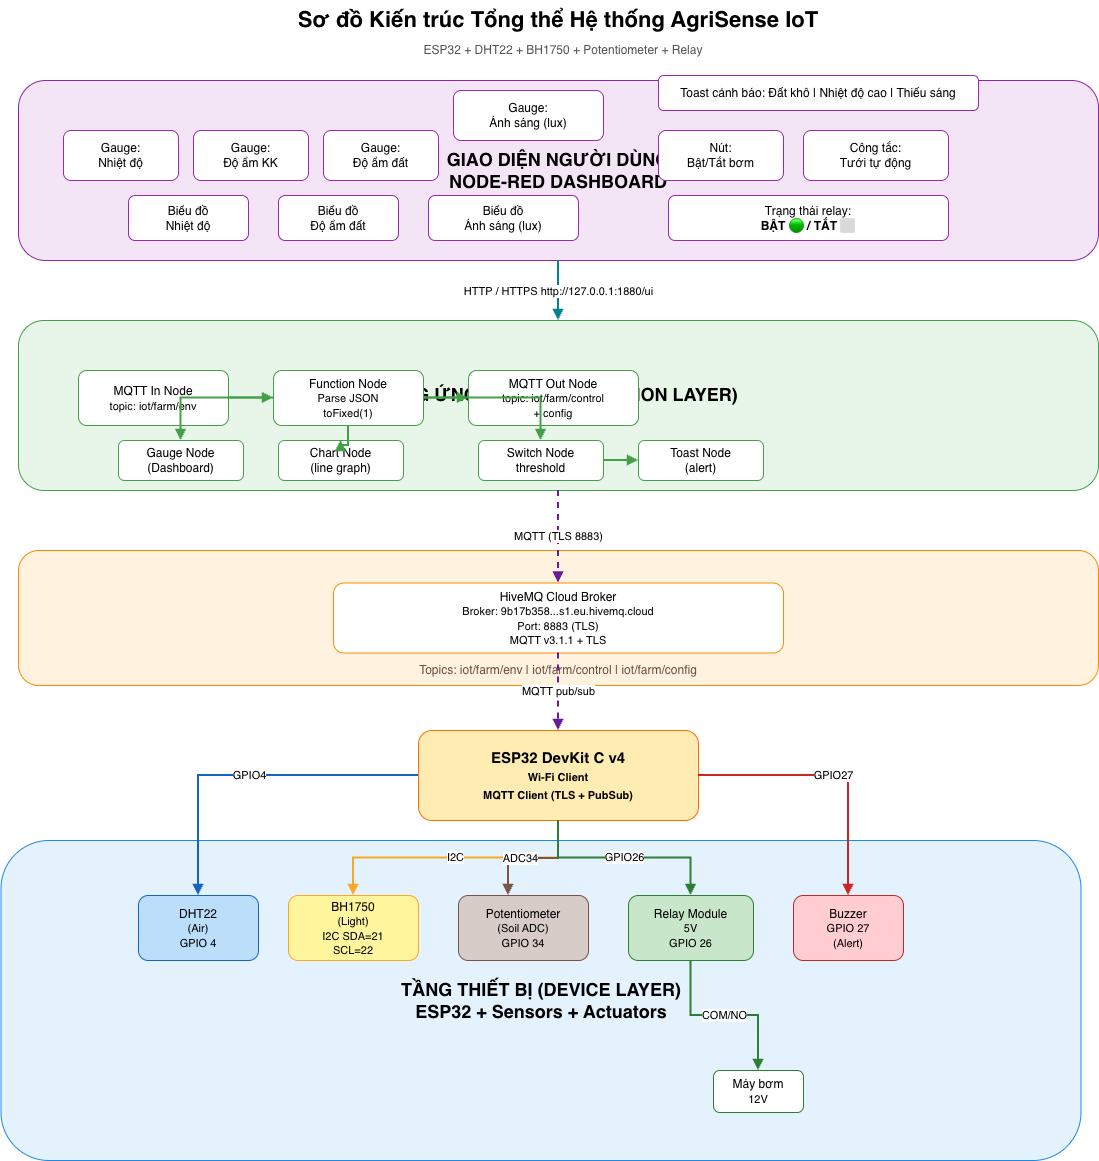
\includegraphics[width=0.65\linewidth]{luu-do-thuat-toan.png}
  \caption{Lưu đồ thuật toán trên ESP32}
  \label{fig:luudo}
\end{figure}

Sơ đồ flow xử lý trên Node-RED:

\begin{figure}[H]
  \centering
  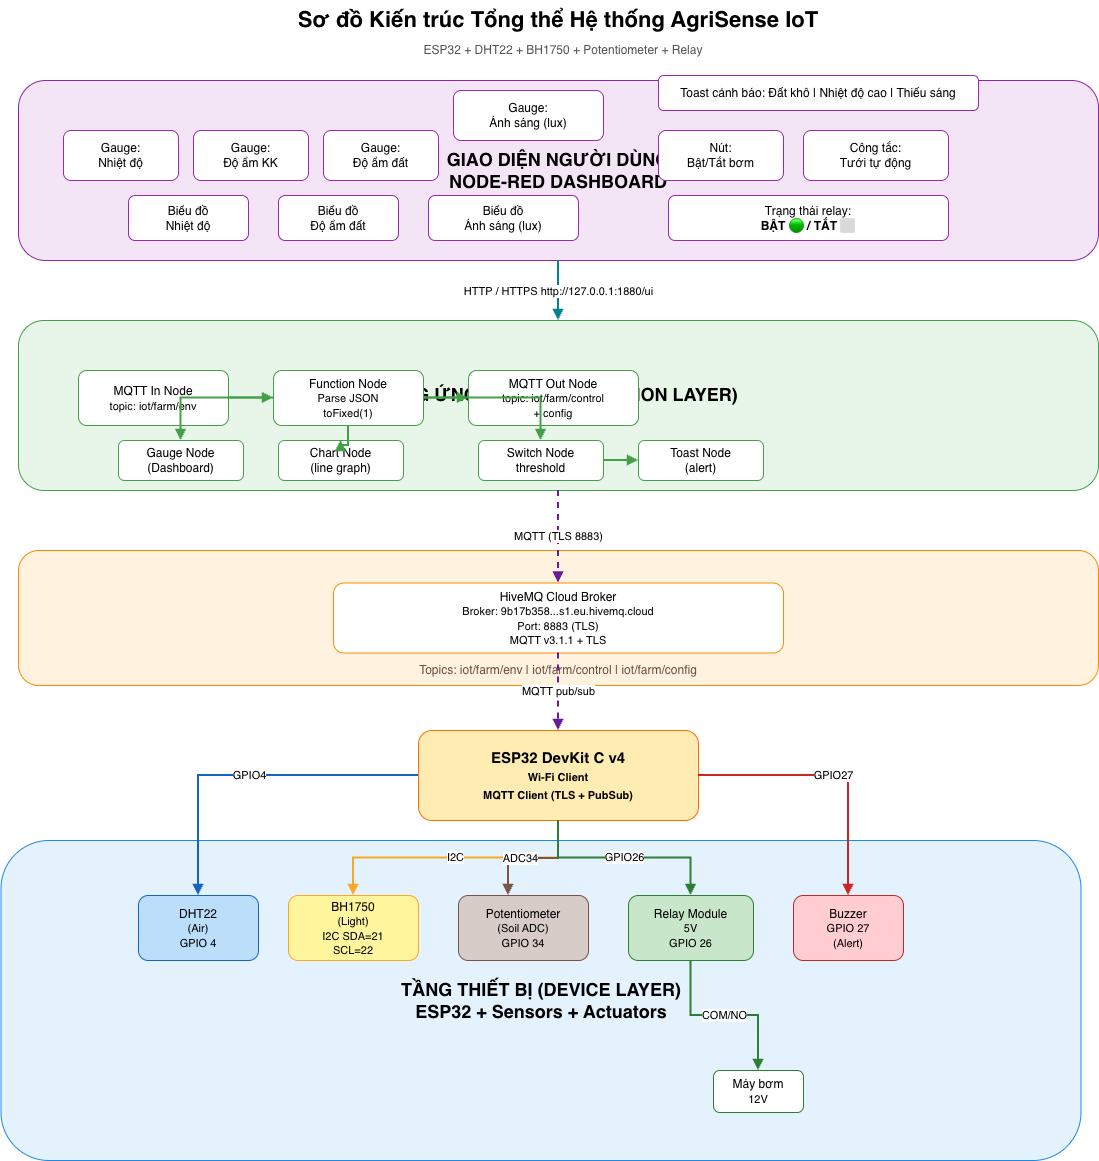
\includegraphics[width=0.9\linewidth]{so-do-flow-nodered.png}
  \caption{Sơ đồ flow xử lý dữ liệu trên Node-RED}
  \label{fig:flow}
\end{figure}

% =============================================================================
% PHẦN 3: CÀI ĐẶT HỆ THỐNG
% =============================================================================
\section{Cài đặt hệ thống}
\label{sec:caidat}

Hướng dẫn từng bước để thiết lập môi trường phát triển, nạp firmware và chạy toàn bộ hệ thống.

\subsection{Công cụ sử dụng}

\begin{table}[H]
  \centering
  \caption{Danh sách công cụ phần mềm sử dụng}
  \label{tbl:tools}
  \begin{tabular}{|L{5cm}|C{4cm}|C{4cm}|}
    \hline
    \textbf{Công cụ} & \textbf{Phiên bản} & \textbf{Ghi chú} \\
    \hline
    \textbf{PlatformIO IDE} (VS Code) & Mới nhất & Biên dịch và nạp firmware ESP32 \\
    \hline
    \textbf{Node.js} & 18.x LTS trở lên & Chạy Node-RED \\
    \hline
    \textbf{Node-RED} & 3.x & Xử lý flow và Dashboard \\
    \hline
    \textbf{node-red-dashboard} & 3.6.x & Giao diện giám sát và điều khiển \\
    \hline
    \textbf{Wokwi} (VS Code extension) & Mới nhất & Mô phỏng phần cứng ESP32 \\
    \hline
    \textbf{HiveMQ Cloud} & Free Tier & MQTT Broker (TLS, port 8883) \\
    \hline
  \end{tabular}
\end{table}

\subsection{Cài đặt PlatformIO cho ESP32}

\textbf{Bước 1 — Cài đặt VS Code và PlatformIO:}

Truy cập \url{https://code.visualstudio.com/}, tải và cài đặt VS Code. Sau đó cài PlatformIO IDE: vào Extensions ($\rightarrow$) tìm \textbf{PlatformIO IDE}, nhấn Install.

\textbf{Bước 2 — Mở project:}

Mở thư mục project chứa \file{platformio.ini} trong VS Code.

\textbf{Bước 3 — Cấu hình Wi-Fi:}

Mở file \file{src/main.cpp}, chỉnh sửa thông tin Wi-Fi:

\begin{lstlisting}[style=ccode, caption={Cấu hình Wi-Fi trong main.cpp}, label={lst:wifi}]
// Môi trường Wokwi: SSID = "WOKWI-GUEST", không cần password
// Môi trường thực tế:
const char *WIFI_SSID = "YOUR_WIFI_SSID";
const char *WIFI_PASSWORD = "YOUR_WIFI_PASSWORD";
\end{lstlisting}

\textbf{Bước 4 — Cấu hình MQTT:}

Thông tin MQTT đã được cấu hình sẵn trong code (HiveMQ Cloud). Nếu cần thay đổi:

\begin{lstlisting}[style=ccode, caption={Cấu hình MQTT trong main.cpp}, label={lst:mqtt}]
const char *MQTT_BROKER = "b1c8f2cc5cd4416fb74b671a407dc0ff.s1.eu.hivemq.cloud";
const int MQTT_PORT = 8883;
const char *MQTT_CLIENT_ID = "esp32-agrisense-01";
const char *MQTT_USERNAME = "hivemq.webclient.1775680760112";
const char *MQTT_PASSWORD = "amy&f0VPG3c5<8,U>qAB";
\end{lstlisting}

\textbf{Bước 5 — Build firmware:}

Mở terminal trong VS Code, chạy:

\begin{itemize}
  \item \code{pio run -e wokwi} — build cho môi trường Wokwi (mô phỏng).
  \item \code{pio run -e esp32dev} — build cho phần cứng thật.
\end{itemize}

Sau khi build thành công, file firmware sẽ nằm ở \file{.pio/build/wokwi/firmware.bin}.

\textbf{Bước 6 — Chạy mô phỏng Wokwi:}

Trong VS Code, nhấn phím \textbf{F5} hoặc biểu tượng Wokwi để khởi chạy mô phỏng. Đảm bảo file \file{wokwi.toml} và \file{diagram.json} nằm cùng thư mục gốc với \file{platformio.ini}.

\subsection{Cài đặt Node-RED}

\textbf{Bước 1 — Cài Node.js:}

Tải và cài \textbf{Node.js LTS} từ \url{https://nodejs.org/}.

\textbf{Bước 2 — Cài Node-RED:}

\begin{lstlisting}[style=bashcode, language=bash, caption={Cài đặt Node-RED}, label={lst:nr}]
npm install -g --unsafe-perm node-red
\end{lstlisting}

\textbf{Bước 3 — Chạy Node-RED:}

\begin{lstlisting}[style=bashcode, language=bash, caption={Chạy Node-RED}, label={lst:nrrun}]
node-red
\end{lstlisting}

Khi khởi động thành công, terminal hiển thị:

\begin{verbatim}
Welcome to Node-RED
...
Server now running at http://127.0.0.1:1880/
\end{verbatim}

Mở trình duyệt tại \url{http://127.0.0.1:1880}.

\textbf{Bước 4 — Cài node-red-dashboard:}

Trong giao diện Node-RED: nhấn \textbf{☰ $\rightarrow$ Manage Palette $\rightarrow$ Install}, tìm \textbf{node-red-dashboard}, nhấn Install. Phiên bản flow tương thích với \textbf{node-red-dashboard 3.6.x}.

\textbf{Bước 5 — Import flow:}

Nhấn \textbf{☰ $\rightarrow$ Import}, paste nội dung file \file{node-red.json}, nhấn Import, sau đó nhấn Deploy.

\subsection{Cấu hình MQTT Broker trong Node-RED}

\begin{enumerate}[label=\arabic*., leftmargin=1.5cm]
  \item Trong editor Node-RED, nhấn đúp vào node \textbf{mqtt-broker} (trong danh sách node bên trái hoặc trong flow).
  \item Điền các trường cấu hình:
\end{enumerate}

\begin{table}[H]
  \centering
  \caption{Cấu hình MQTT broker trong Node-RED}
  \label{tbl:broker}
  \begin{tabular}{|L{3.5cm}|C{4cm}|C{5cm}|}
    \hline
    \textbf{Trường} & \textbf{Giá trị} & \textbf{Ghi chú} \\
    \hline
    \textbf{Server} & \codebreak{b1c8f2cc5cd4416fb74b671a407dc0ff.s1.eu.hivemq.cloud} & HiveMQ Cloud hostname \\
    \hline
    \textbf{Port} & \textbf{8883} & TLS \\
    \hline
    \textbf{Use TLS} & Bật & Mã hóa end-to-end \\
    \hline
    \textbf{Username} & \code{****} & Tài khoản HiveMQ thật \\
    \hline
    \textbf{Password} & \code{****} & Mật khẩu HiveMQ thật \\
    \hline
    \textbf{Protocol Level} & MQTT v3.1.1 (4) & \\
    \hline
  \end{tabular}
\end{table}

Nhấn Update $\rightarrow$ Deploy.

\subsection{Truy cập Dashboard và kiểm tra kết nối}

\begin{itemize}
  \item Truy cập Dashboard: \url{http://127.0.0.1:1880/ui}
  \item Đảm bảo ESP32 đang chạy (Wokwi hoặc phần cứng thật).
  \item Kiểm tra gauge cập nhật mỗi $\sim$5 giây.
  \item Thử nhấn nút Bật/Tắt bơm trên Dashboard.
  \item Xem Serial Monitor (115200 baud) để kiểm tra log.
\end{itemize}

\begin{figure}[H]
  \centering
  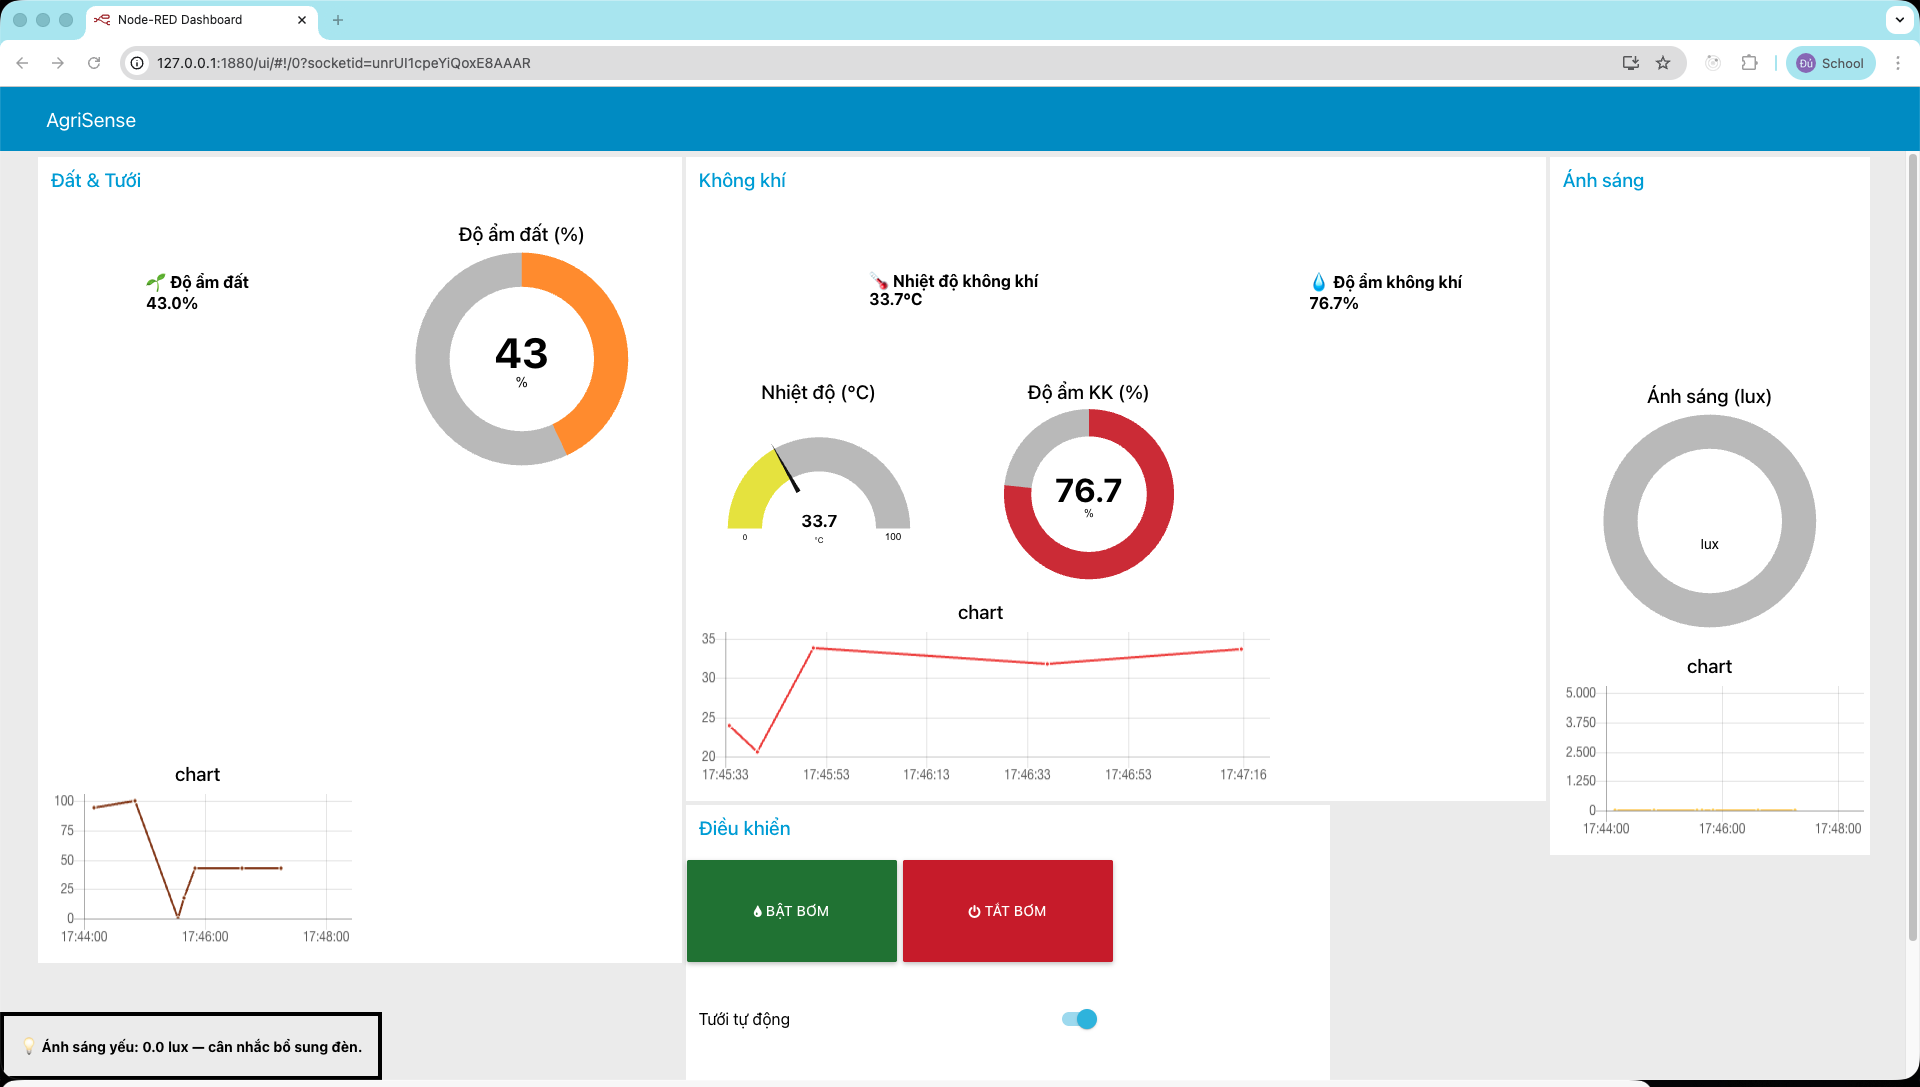
\includegraphics[width=0.9\linewidth]{nodered-dashboard-full.png}
  \caption{Giao diện Dashboard Node-RED: gauge độ ẩm đất, nhiệt độ, độ ẩm KK và điều khiển bơm}
  \label{fig:nr-dash}
\end{figure}

\begin{figure}[H]
  \centering
  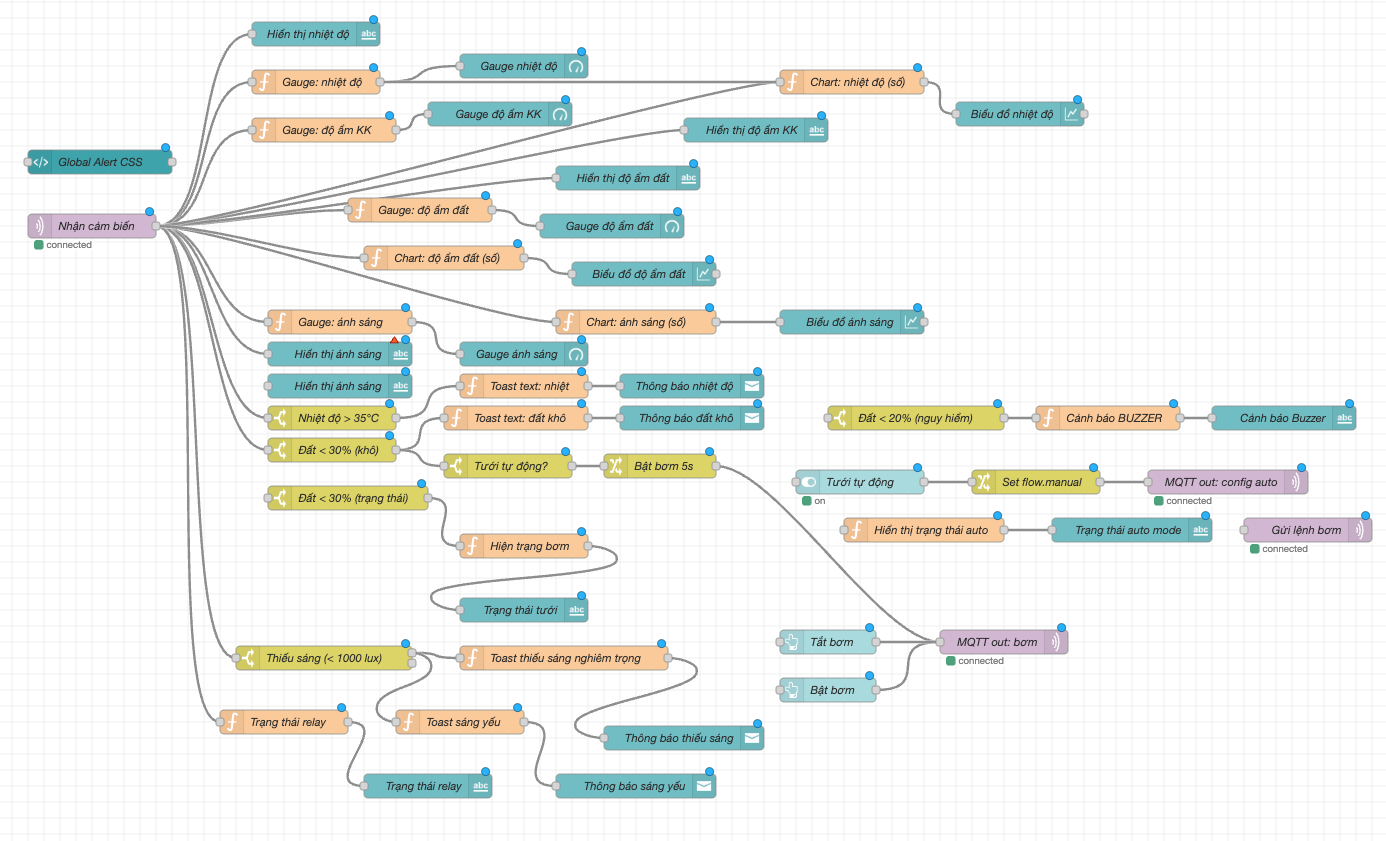
\includegraphics[width=0.9\linewidth]{nodered-flow-full.png}
  \caption{Giao diện editor Node-RED với flow đầy đủ}
  \label{fig:nr-flow}
\end{figure}

% =============================================================================
% PHẦN 4: KẾT QUẢ THỰC HIỆN
% =============================================================================
\section{Kết quả thực hiện}
\label{sec:ketqua}

\subsection{Kết quả giám sát môi trường}

Hệ thống hoạt động ổn định với chu kỳ đọc dữ liệu 5 giây. Mỗi lần đọc, DHT22 đo nhiệt độ và độ ẩm không khí, Potentiometer cung cấp giá trị ADC để tính độ ẩm đất, ESP32 đóng gói thành chuỗi JSON và publish lên topic \code{iot/farm/env}. JSON payload có cấu trúc:

\begin{lstlisting}[style=jcode, caption={JSON payload gửi lên topic iot/farm/env}, label={lst:json}]
{
  "device": "AgriSense-01",
  "temperature": 25.3,
  "humidity": 60.2,
  "soilMoisture": 45.0,
  "pumpStatus": false,
  "timestamp": 12345678
}
\end{lstlisting}

Node-RED nhận JSON, parse và phân luồng tới các node hiển thị. Gauge độ ẩm đất (dạng donut) hiển thị giá trị với ba vùng màu: đỏ (0--30\%: khô), cam (30--60\%: trung bình), xanh (60--100\%: ẩm). Biểu đồ line vẽ điểm mới mỗi 5 giây, tự động xóa điểm cũ sau 1 giờ (\code{removeOlderPoints: 10}, \code{removeOlderUnit: 3600}), đảm bảo biểu đồ không bị quá tải.

Gauge nhiệt độ hiển thị giá trị với kim chỉ vị trí tương ứng trên thang 0--100$^\circ$C, tự động đổi màu theo ngưỡng (xanh: dưới 33, vàng: 33--67, đỏ: trên 67). Gauge độ ẩm không khí dạng donut với ngưỡng tương tự.

\subsection{Kết quả cảnh báo}

Khi độ ẩm đất giảm xuống dưới 30\% (ngưỡng khô), hệ thống thực hiện hai hành động đồng thời: (1) ESP32 gọi \code{beepAlert(2, 150, 150)} — buzzer bíp 2 lần ngắn để cảnh báo tại chỗ; (2) Node-RED hiển thị toast thông báo \code{🌵 Đất khô: XX\% — cần tưới} tại góc dưới bên trái Dashboard trong 8 giây.

Khi độ ẩm đất giảm xuống dưới 20\% (ngưỡng nguy hiểm), buzzer bíp 5 lần liên tục (mỗi lần 300ms bật, 200ms tắt), và Node-RED hiển thị cảnh báo đỏ trên Dashboard với nội dung \code{🔔 CẢNH BÁO: Đất khô nghiêm trọng (XX\%) — Bật BUZZER trên thiết bị!}.

Ngưỡng cảnh báo được lựa chọn dựa trên điều kiện thực tế trồng cây: đất có độ ẩm dưới 30\% được coi là khô cần tưới; dưới 20\% là ngưỡng nguy hiểm, cây có thể bị héo nếu không được tưới kịp thời.

Khi nhiệt độ không khí vượt ngưỡng 35$^\circ$C, toast thông báo \code{⚠️ Nhiệt độ cao: XX.X°C} được hiển thị. Ngưỡng này được chọn vì nhiệt độ trên 35$^\circ$C có thể gây stress nhiệt cho cây trồng.

\subsection{Kết quả điều khiển bơm từ Dashboard}

Người dùng có thể bật/tắt máy bơm (LED mô phỏng) bằng hai cách:

\textbf{Cách 1 — Bật/tắt thủ công:} Nhấn nút \textbf{Bật bơm} (màu xanh) hoặc \textbf{Tắt bơm} (màu đỏ) trên Dashboard. Node-RED gửi JSON \code{\{"pump":true,"duration":5\}} hoặc \code{\{"pump":false,"duration":0\}} lên topic \code{iot/farm/control}. ESP32 nhận lệnh qua \code{mqttCallback()}, LED bật (HIGH) hoặc tắt (LOW) tại chân GPIO 5.

\textbf{Cách 2 — Tưới tự động:} Bật công tắc \textbf{Tưới tự động} trên Dashboard. Khi độ ẩm đất $<$ 30\%, hệ thống tự động gửi lệnh bật bơm mà không cần can thiệp thủ công. Tính năng này đảm bảo cây luôn được tưới kịp thời khi độ ẩm giảm xuống dưới ngưỡng an toàn.

\begin{figure}[H]
  \centering
  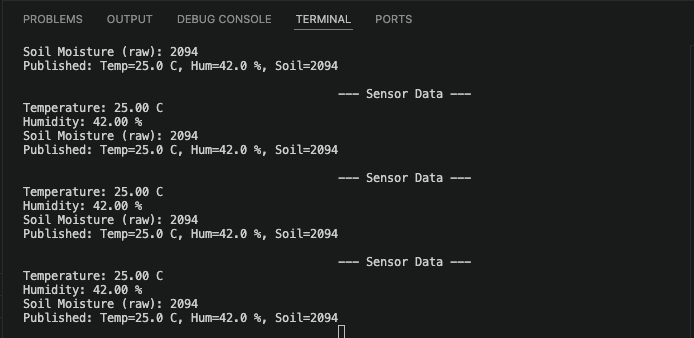
\includegraphics[width=0.85\linewidth]{serial-monitor.png}
  \caption{Serial Monitor: log dữ liệu cảm biến và trạng thái MQTT trên PlatformIO}
  \label{fig:serial}
\end{figure}

\subsection{Tổng hợp các chức năng đã triển khai}

\begin{table}[H]
  \centering
  \caption{Tổng hợp các chức năng đã triển khai}
  \label{tbl:chucnang}
  \begin{tabular}{|L{4cm}|C{3cm}|C{4.5cm}|}
    \hline
    \textbf{Chức năng} & \textbf{Trạng thái} & \textbf{Ghi chú} \\
    \hline
    Đọc DHT22 mỗi 5 giây & Hoàn thành & GPIO 4, fallback random khi lỗi \\
    \hline
    Đọc Potentiometer (độ ẩm đất) & Hoàn thành & GPIO 34, ADC 12-bit, map 0--100\% \\
    \hline
    Truyền MQTT (TLS port 8883) & Hoàn thành & WiFiClientSecure + PubSubClient \\
    \hline
    Hiển thị Gauge độ ẩm đất & Hoàn thành & Donut gauge, 3 vùng màu đỏ/cam/xanh \\
    \hline
    Hiển thị Gauge nhiệt độ & Hoàn thành & 3 vùng màu, min=0, max=100 \\
    \hline
    Hiển thị Gauge độ ẩm KK & Hoàn thành & Donut gauge, min=0, max=100 \\
    \hline
    Biểu đồ line thời gian thực & Hoàn thành & dot=true, removeOlderUnit=3600 \\
    \hline
    Buzzer bíp khi đất khô ($<$ 30\%) & Hoàn thành & 2 lần, mỗi lần 150ms \\
    \hline
    Buzzer bíp khi đất nguy hiểm ($<$ 20\%) & Hoàn thành & 5 lần, mỗi lần 300ms \\
    \hline
    Toast cảnh báo đất khô & Hoàn thành & Ngưỡng $<$ 30\%, 8 giây \\
    \hline
    Toast cảnh báo nhiệt độ cao & Hoàn thành & Ngưỡng $>$ 35$^\circ$C, 8 giây \\
    \hline
    Cảnh báo nguy hiểm (đất $<$ 20\%) & Hoàn thành & Hiển thị đỏ trên Dashboard \\
    \hline
    Bật bơm thủ công (button) & Hoàn thành & Gửi JSON lên iot/farm/control \\
    \hline
    Tắt bơm thủ công (button) & Hoàn thành & Gửi JSON lên iot/farm/control \\
    \hline
    Tưới tự động (switch) & Hoàn thành & Bật bơm khi ẩm đất $<$ 30\% \\
    \hline
    Reconnect Wi-Fi tự động & Hoàn thành & Kiểm tra trong loop() \\
    \hline
    Reconnect MQTT non-blocking & Hoàn thành & Thử lại mỗi 5 giây \\
    \hline
    Mô phỏng Wokwi đầy đủ & Hoàn thành & ESP32 + DHT22 + Pot + LED + Buzzer \\
    \hline
  \end{tabular}
\end{table}

% =============================================================================
% PHẦN 5: KẾT LUẬN VÀ HƯỚNG PHÁT TRIỂN
% =============================================================================
\section{Kết luận và hướng phát triển}
\label{sec:ketluan}

\subsection{Các công việc đã thực hiện được}

Qua quá trình nghiên cứu và triển khai, báo cáo đã hoàn thành các mục tiêu đề ra ban đầu. Hệ thống AgriSense IoT đã được thiết kế và triển khai thành công với các kết quả cụ thể sau:

\begin{enumerate}[label=\arabic*., leftmargin=1.5cm]
  \item \textbf{Hệ thống IoT ba tầng hoàn chỉnh:} Tầng thiết bị (ESP32 + DHT22 + Potentiometer) kết nối với tầng trung gian (HiveMQ Cloud TLS) và tầng ứng dụng (Node-RED Dashboard), hoạt động ổn định trong điều kiện thực tế.
  \item \textbf{Giám sát ba thông số môi trường:} Nhiệt độ không khí, độ ẩm không khí và độ ẩm đất được thu thập và truyền lên cloud mỗi 5 giây qua giao thức MQTT, với JSON payload được định dạng chuẩn, dễ xử lý và mở rộng.
  \item \textbf{Giao diện Dashboard trực quan:} Cho phép giám sát ba thông số theo thời gian thực qua gauge và biểu đồ line, cung cấp cái nhìn tổng quan về điều kiện môi trường trồng cây.
  \item \textbf{Hệ thống cảnh báo đa tầng:} Buzzer báo động tại chỗ (ESP32) kết hợp toast thông báo trên Dashboard khi độ ẩm đất giảm xuống dưới ngưỡng, giúp người dùng phản ứng kịp thời.
  \item \textbf{Điều khiển bơm linh hoạt:} Chế độ bật/tắt thủ công và chế độ tưới tự động dựa trên ngưỡng độ ẩm đất, mang lại sự linh hoạt cao trong vận hành.
  \item \textbf{Toàn bộ hệ thống mô phỏng thành công trên Wokwi:} Cho phép kiểm thử mà không cần phần cứng thật, với đầy đủ sơ đồ kết nối và firmware.
\end{enumerate}

Hệ thống có thể được ứng dụng thực tế trong việc giám sát và tưới cây trong nhà kính, trồng rau thủy canh, trồng cây trên ban công hoặc sân thượng đô thị.

\subsection{Các công việc chưa thực hiện được}

\begin{enumerate}[label=\arabic*., leftmargin=1.5cm]
  \item \textbf{Xác thực chứng chỉ TLS đầy đủ (\code{setCACert}):} Hiện tại đang dùng \code{espClient.setInsecure()} — bỏ qua xác thực certificate. Phù hợp cho môi trường demo nhưng chưa đạt tiêu chuẩn production.
  \item \textbf{Relay và máy bơm thực sự:} LED chỉ là mô phỏng, chưa kết nối relay 5V và máy bơm nước 12V thực sự để hệ thống thực sự tưới cây.
  \item \textbf{Lưu trữ dữ liệu dài hạn (database):} Chưa có cơ chế lưu trữ dữ liệu lịch sử ngoài biểu đồ real-time trên Dashboard. Có thể bổ sung InfluxDB hoặc MySQL.
  \item \textbf{Xác thực người dùng trên Dashboard:} NRD mặc định không có login, bất kỳ ai truy cập URL đều có thể điều khiển.
  \item \textbf{OTA (Over-The-Air) cập nhật firmware:} Chưa triển khai cập nhật firmware từ xa qua Wi-Fi.
\end{enumerate}

\subsection{Hướng phát triển tiếp theo}

Dựa trên kết quả nghiên cứu và hạn chế của hệ thống hiện tại, các hướng phát triển tiếp theo được đề xuất:

\begin{enumerate}[label=\arabic*., leftmargin=1.5cm]
  \item \textbf{Triển khai phần cứng thực:} Thay Potentiometer bằng cảm biến độ ẩm đất capacitive (vỉ FY-550 hoặc vỉ với IC v3), kết nối relay 5V và máy bơm nước 12V để hệ thống thực sự tưới cây.
  \item \textbf{Nâng cấp bảo mật TLS:} Sử dụng chứng chỉ CA hợp lệ thay vì \code{setInsecure()}, đảm bảo hệ thống an toàn khi triển khai thực tế.
  \item \textbf{Triển khai lưu trữ dữ liệu dài hạn:} Thêm InfluxDB hoặc MySQL để lưu trữ dữ liệu lịch sử, phân tích xu hướng theo ngày, tuần, tháng, và xuất báo cáo.
  \item \textbf{Xác thực Dashboard:} Bật \code{adminAuth} trong \code{settings.js} của Node-RED để yêu cầu đăng nhập trước khi truy cập.
  \item \textbf{OTA cập nhật firmware:} Triển khai cập nhật firmware từ xa qua Wi-Fi để thuận tiện cho việc bảo trì và nâng cấp.
  \item \textbf{Mở rộng cảm biến:} Bổ sung cảm biến ánh sáng (BH1750), cảm biến độ pH đất, cảm biến mực nước bể để hệ thống giám sát toàn diện hơn.
\end{enumerate}

% =============================================================================
% TÀI LIỆU THAM KHẢO
% =============================================================================
\newpage
\section*{Tài liệu tham khảo}
\addcontentsline{toc}{section}{Tài liệu tham khảo}

\begin{enumerate}[label={[\arabic*]}, leftmargin=*, itemsep=4pt]
  \item Espressif Systems. \textit{ESP32 Series Datasheet}. Truy cập: \url{https://www.espressif.com/sites/default/files/documentation/esp32_datasheet_en.pdf}.
  \item Node-RED. \textit{Node-RED Documentation}. IBM \& others. Truy cập: \url{https://nodered.org/docs/}.
  \item HiveMQ. \textit{HiveMQ Cloud}. Truy cập: \url{https://www.hivemq.com/cloud/}.
  \item Adafruit. \textit{DHT sensor library for Arduino}. Truy cập: \url{https://github.com/adafruit/DHT-sensor-library}.
  \item Nick O'Leary. \textit{PubSubClient for Arduino}. Truy cập: \url{https://github.com/knolleary/pubsubclient}.
  \item Node-RED. \textit{node-red-dashboard}. Truy cập: \url{https://flows.nodered.org/node/node-red-dashboard}.
  \item Wokwi. \textit{Wokwi ESP32 Simulator}. Truy cập: \url{https://wokwi.com/}.
  \item PlatformIO. \textit{PlatformIO Documentation}. Truy cập: \url{https://docs.platformio.org/}.
\end{enumerate}

% =============================================================================
% CÁC PHỤ LỤC
% =============================================================================
\newpage
\pagenumbering{gobble}

\begin{center}
  {\large\bfseries CÁC PHỤ LỤC}\\
  \textit{(Không tính vào số trang của bản báo cáo)}
\end{center}
\vspace{0.5cm}

% ----- PHỤ LỤC A -----
\subsection*{PHỤ LỤC A. Mã nguồn chương trình ESP32}
\addcontentsline{toc}{subsection}{Phụ lục A. Mã nguồn chương trình ESP32}
\label{sec:pl-a}

\textbf{Lưu ý:} Trước khi nạp firmware, cần cập nhật các thông tin sau trong code: \code{WIFI_SSID} và \code{WIFI_PASSWORD} (tên và mật khẩu Wi-Fi); \code{MQTT_USERNAME} và \code{MQTT_PASSWORD} (tài khoản HiveMQ Cloud). Thông tin xác thực MQTT đã được ẩn trong tài liệu này vì lý do bảo mật.

\textbf{Các bước nạp firmware:}

\begin{enumerate}[label=\arabic*., leftmargin=1.5cm]
  \item Mở project trong PlatformIO IDE (VS Code).
  \item Chạy \code{pio run -e wokwi} để build firmware cho Wokwi.
  \item Nhấn F5 hoặc biểu tượng Wokwi để chạy mô phỏng.
  \item Hoặc chạy \code{pio run -e esp32dev \&\& pio run -e esp32dev --target upload} để nạp firmware lên ESP32 thật.
\end{enumerate}

\IfFileExists{main-src.txt}{%
  \lstinputlisting[
    style=ccode,
    caption={Firmware ESP32 — main.cpp},
    label={lst:pl-arduino}
  ]{main-src.txt}%
}{%
  \textbf{Lưu ý:} File \file{main-src.txt} chưa được tạo. Sao chép nội dung file \file{src/main.cpp} vào \file{main-src.txt} rồi đặt cùng thư mục với \file{main.tex} để hiển thị mã nguồn.
}

% ----- PHỤ LỤC B -----
\subsection*{PHỤ LỤC B. Mã nguồn Node-RED (JSON Flow)}
\addcontentsline{toc}{subsection}{Phụ lục B. Mã nguồn Node-RED (JSON Flow)}
\label{sec:pl-b}

\textbf{Các bước import flow vào Node-RED:}

\begin{enumerate}[label=\arabic*., leftmargin=1.5cm]
  \item Truy cập Node-RED tại \url{http://127.0.0.1:1880}.
  \item Nhấn Menu $\rightarrow$ Import.
  \item Chọn thẻ Clipboard, paste toàn bộ nội dung JSON bên dưới.
  \item Nhấn Import để thêm flow.
  \item Nhấn Deploy (nút đỏ góc phải) để chạy flow.
\end{enumerate}

\textbf{Lưu ý:} Sau khi import, kiểm tra và cập nhật cấu hình node \textbf{mqtt-broker}: hostname, port (8883), username, password phải khớp với tài khoản HiveMQ Cloud đang sử dụng.

\IfFileExists{node-red-flow.txt}{%
  \lstinputlisting[
    style=jcode,
    caption={Node-RED Flow (JSON) — node-red.json},
    label={lst:pl-nodered}
  ]{node-red-flow.txt}%
}{%
  \textbf{Lưu ý:} File \file{node-red-flow.txt} chưa được tạo. Sao chép nội dung file \file{node-red.json} vào \file{node-red-flow.txt} rồi đặt cùng thư mục với \file{main.tex} để hiển thị flow.
}

% ----- PHỤ LỤC C -----
\subsection*{PHỤ LỤC C. Mã nguồn sơ đồ Wokwi (JSON)}
\addcontentsline{toc}{subsection}{Phụ lục C. Mã nguồn sơ đồ Wokwi (JSON)}
\label{sec:pl-c}

\textbf{Các bước mở sơ đồ mạch trên Wokwi:}

\begin{enumerate}[label=\arabic*., leftmargin=1.5cm]
  \item Truy cập \url{https://wokwi.com/}.
  \item Đăng nhập (hoặc tạo tài khoản mới).
  \item Tạo project mới hoặc import file JSON bên dưới.
  \item Nhấn Play để chạy mô phỏng.
\end{enumerate}

\IfFileExists{wokwi-diagram.txt}{%
  \lstinputlisting[
    style=jcode,
    caption={Sơ đồ mạch Wokwi (JSON) — diagram.json},
    label={lst:pl-wokwi}
  ]{wokwi-diagram.txt}%
}{%
  \textbf{Lưu ý:} File \file{wokwi-diagram.txt} chưa được tạo. Sao chép nội dung file \file{diagram.json} vào \file{wokwi-diagram.txt} rồi đặt cùng thư mục với \file{main.tex} để hiển thị sơ đồ.
}

% =============================================================================
\end{document}
